% Options for packages loaded elsewhere
% Options for packages loaded elsewhere
\PassOptionsToPackage{unicode}{hyperref}
\PassOptionsToPackage{hyphens}{url}
%
\documentclass[
  10pt,
  letterpaper,
  DIV=11,
  numbers=noendperiod,
  twoside]{scrartcl}
\usepackage{xcolor}
\usepackage[left=1in, right=1in, top=0.8in, bottom=0.8in,
paperheight=9.5in, paperwidth=6.5in, includemp=TRUE, marginparwidth=0in,
marginparsep=0in]{geometry}
\usepackage{amsmath,amssymb}
\setcounter{secnumdepth}{5}
\usepackage{iftex}
\ifPDFTeX
  \usepackage[T1]{fontenc}
  \usepackage[utf8]{inputenc}
  \usepackage{textcomp} % provide euro and other symbols
\else % if luatex or xetex
  \usepackage{unicode-math} % this also loads fontspec
  \defaultfontfeatures{Scale=MatchLowercase}
  \defaultfontfeatures[\rmfamily]{Ligatures=TeX,Scale=1}
\fi
\usepackage{lmodern}
\ifPDFTeX\else
  % xetex/luatex font selection
  \setmainfont[ItalicFont=EB Garamond Italic,BoldFont=EB Garamond
Bold]{EB Garamond Math}
  \setsansfont[]{Europa-Bold}
  \setmathfont[]{Garamond-Math}
\fi
% Use upquote if available, for straight quotes in verbatim environments
\IfFileExists{upquote.sty}{\usepackage{upquote}}{}
\IfFileExists{microtype.sty}{% use microtype if available
  \usepackage[]{microtype}
  \UseMicrotypeSet[protrusion]{basicmath} % disable protrusion for tt fonts
}{}
\usepackage{setspace}
% Make \paragraph and \subparagraph free-standing
\makeatletter
\ifx\paragraph\undefined\else
  \let\oldparagraph\paragraph
  \renewcommand{\paragraph}{
    \@ifstar
      \xxxParagraphStar
      \xxxParagraphNoStar
  }
  \newcommand{\xxxParagraphStar}[1]{\oldparagraph*{#1}\mbox{}}
  \newcommand{\xxxParagraphNoStar}[1]{\oldparagraph{#1}\mbox{}}
\fi
\ifx\subparagraph\undefined\else
  \let\oldsubparagraph\subparagraph
  \renewcommand{\subparagraph}{
    \@ifstar
      \xxxSubParagraphStar
      \xxxSubParagraphNoStar
  }
  \newcommand{\xxxSubParagraphStar}[1]{\oldsubparagraph*{#1}\mbox{}}
  \newcommand{\xxxSubParagraphNoStar}[1]{\oldsubparagraph{#1}\mbox{}}
\fi
\makeatother


\usepackage{longtable,booktabs,array}
\usepackage{calc} % for calculating minipage widths
% Correct order of tables after \paragraph or \subparagraph
\usepackage{etoolbox}
\makeatletter
\patchcmd\longtable{\par}{\if@noskipsec\mbox{}\fi\par}{}{}
\makeatother
% Allow footnotes in longtable head/foot
\IfFileExists{footnotehyper.sty}{\usepackage{footnotehyper}}{\usepackage{footnote}}
\makesavenoteenv{longtable}
\usepackage{graphicx}
\makeatletter
\newsavebox\pandoc@box
\newcommand*\pandocbounded[1]{% scales image to fit in text height/width
  \sbox\pandoc@box{#1}%
  \Gscale@div\@tempa{\textheight}{\dimexpr\ht\pandoc@box+\dp\pandoc@box\relax}%
  \Gscale@div\@tempb{\linewidth}{\wd\pandoc@box}%
  \ifdim\@tempb\p@<\@tempa\p@\let\@tempa\@tempb\fi% select the smaller of both
  \ifdim\@tempa\p@<\p@\scalebox{\@tempa}{\usebox\pandoc@box}%
  \else\usebox{\pandoc@box}%
  \fi%
}
% Set default figure placement to htbp
\def\fps@figure{htbp}
\makeatother


% definitions for citeproc citations
\NewDocumentCommand\citeproctext{}{}
\NewDocumentCommand\citeproc{mm}{%
  \begingroup\def\citeproctext{#2}\cite{#1}\endgroup}
\makeatletter
 % allow citations to break across lines
 \let\@cite@ofmt\@firstofone
 % avoid brackets around text for \cite:
 \def\@biblabel#1{}
 \def\@cite#1#2{{#1\if@tempswa , #2\fi}}
\makeatother
\newlength{\cslhangindent}
\setlength{\cslhangindent}{1.5em}
\newlength{\csllabelwidth}
\setlength{\csllabelwidth}{3em}
\newenvironment{CSLReferences}[2] % #1 hanging-indent, #2 entry-spacing
 {\begin{list}{}{%
  \setlength{\itemindent}{0pt}
  \setlength{\leftmargin}{0pt}
  \setlength{\parsep}{0pt}
  % turn on hanging indent if param 1 is 1
  \ifodd #1
   \setlength{\leftmargin}{\cslhangindent}
   \setlength{\itemindent}{-1\cslhangindent}
  \fi
  % set entry spacing
  \setlength{\itemsep}{#2\baselineskip}}}
 {\end{list}}
\usepackage{calc}
\newcommand{\CSLBlock}[1]{\hfill\break\parbox[t]{\linewidth}{\strut\ignorespaces#1\strut}}
\newcommand{\CSLLeftMargin}[1]{\parbox[t]{\csllabelwidth}{\strut#1\strut}}
\newcommand{\CSLRightInline}[1]{\parbox[t]{\linewidth - \csllabelwidth}{\strut#1\strut}}
\newcommand{\CSLIndent}[1]{\hspace{\cslhangindent}#1}



\setlength{\emergencystretch}{3em} % prevent overfull lines

\providecommand{\tightlist}{%
  \setlength{\itemsep}{0pt}\setlength{\parskip}{0pt}}



 


\setlength\heavyrulewidth{0ex}
\setlength\lightrulewidth{0ex}
\usepackage[automark]{scrlayer-scrpage}
\clearpairofpagestyles
\cehead{
  Anon
  }
\cohead{
  The End of Decision Theory
  }
\ohead{\bfseries \pagemark}
\cfoot{}
\makeatletter
\newcommand*\NoIndentAfterEnv[1]{%
  \AfterEndEnvironment{#1}{\par\@afterindentfalse\@afterheading}}
\makeatother
\NoIndentAfterEnv{itemize}
\NoIndentAfterEnv{enumerate}
\NoIndentAfterEnv{description}
\NoIndentAfterEnv{quote}
\NoIndentAfterEnv{equation}
\NoIndentAfterEnv{longtable}
\NoIndentAfterEnv{abstract}
\renewenvironment{abstract}
 {\vspace{-1.25cm}
 \quotation\small\noindent\rule{\linewidth}{.5pt}\par\smallskip
 \noindent }
 {\par\noindent\rule{\linewidth}{.5pt}\endquotation}
\setlength\heavyrulewidth{0ex}
\setlength\lightrulewidth{0ex}
\KOMAoption{captions}{tableheading}
\makeatletter
\@ifpackageloaded{caption}{}{\usepackage{caption}}
\AtBeginDocument{%
\ifdefined\contentsname
  \renewcommand*\contentsname{Table of contents}
\else
  \newcommand\contentsname{Table of contents}
\fi
\ifdefined\listfigurename
  \renewcommand*\listfigurename{List of Figures}
\else
  \newcommand\listfigurename{List of Figures}
\fi
\ifdefined\listtablename
  \renewcommand*\listtablename{List of Tables}
\else
  \newcommand\listtablename{List of Tables}
\fi
\ifdefined\figurename
  \renewcommand*\figurename{Figure}
\else
  \newcommand\figurename{Figure}
\fi
\ifdefined\tablename
  \renewcommand*\tablename{Table}
\else
  \newcommand\tablename{Table}
\fi
}
\@ifpackageloaded{float}{}{\usepackage{float}}
\floatstyle{ruled}
\@ifundefined{c@chapter}{\newfloat{codelisting}{h}{lop}}{\newfloat{codelisting}{h}{lop}[chapter]}
\floatname{codelisting}{Listing}
\newcommand*\listoflistings{\listof{codelisting}{List of Listings}}
\makeatother
\makeatletter
\makeatother
\makeatletter
\@ifpackageloaded{caption}{}{\usepackage{caption}}
\@ifpackageloaded{subcaption}{}{\usepackage{subcaption}}
\makeatother
\usepackage{bookmark}
\IfFileExists{xurl.sty}{\usepackage{xurl}}{} % add URL line breaks if available
\urlstyle{same}
\hypersetup{
  pdftitle={The End of Decision Theory},
  pdfauthor={Anon},
  hidelinks,
  pdfcreator={LaTeX via pandoc}}


\title{The End of Decision Theory}
\author{Anon}
\date{}
\begin{document}
\maketitle


\setstretch{1.1}
\section{What is Decision Theory a Theory
Of?}\label{what-is-decision-theory-a-theory-of}

If you're reading a paper like this, you're probably familiar with
seeing papers defending this or that decision theory. Familiar decision
theories include:

\begin{itemize}
\tightlist
\item
  Causal Decision Theory (\citeproc{ref-GibbardHarper1978}{Gibbard and
  Harper 1978}; \citeproc{ref-Lewis1981b}{Lewis 1981};
  \citeproc{ref-Skyrms1990}{Skyrms 1990}; \citeproc{ref-Joyce1999}{Joyce
  1999});
\item
  Evidential Decision Theory (\citeproc{ref-Ahmed2014}{Ahmed 2014});
\item
  Benchmark theory (\citeproc{ref-Wedgwood2013a}{Wedgwood 2013});
\item
  Risk-Weighted theory (\citeproc{ref-BuchakRisk}{Buchak 2013});
\item
  Tournament Decision Theory (\citeproc{ref-Podgorski2022}{Podgorski
  2022}); and
\item
  Functional Decision Theory
  (\citeproc{ref-LevinsteinSoares2020}{Levinstein and Soares 2020})
\end{itemize}

Other theories haven't had snappy `isms' applied to them, such as the
non-standard version of Causal Decision Theory that Dmitri Gallow
(\citeproc{ref-Gallow2020}{2020}) defends, or the pluralist decision
theory that Jack Spencer (\citeproc{ref-Spencer2021}{2021}) defends, or
the broadly ratificationist theory that Melissa Fusco
(\citeproc{ref-Fusco2024}{2024}) defends.

This paper isn't going to take sides between these nine or more
theories.\footnote{The arguments here are intended to support a theory
  like Fusco's, but in a fairly roundabout way, but the connection
  between what I say here and Fusco's theory would take a paper as long
  as this one to set out.} Rather it is going to ask a prior pair of
questions.

\begin{enumerate}
\def\labelenumi{\arabic{enumi}.}
\tightlist
\item
  If these are the possible answers, what is the question? That is, what
  is the question to which decision theories are possible answers?
\item
  Why is that an interesting question? What do we gain by answering it?
\end{enumerate}

On 1, I will argue that decision theories are answers to a question
about what an ideal decider would do. The `ideal' here is like the
`ideal' in a scientific idealisation, not the ideal in something like an
ideal advisor moral theory. That is, the ideal decider is an
idealisation in the sense of being simple, not in the sense of being
perfect. The ideal decision maker is ideal in the same way that the
point-masses in the ideal gas model are ideal; they are (relatively)
simple to work with. The main opponent I have in mind is someone who
says that in some sense decision theory tells us what decisions we
should make.

On 2, I will argue that the point of asking this question is that these
idealisations play important roles in explanatorily useful models of
social interactions, such as the model of the used car market that
George Akerlof (\citeproc{ref-Akerlof1970}{1970}) described. Here, the
main opponent I have in mind is someone who says that decision theory is
useful because it helps us make better decisions.

There is another pair of answers to this question which is interesting,
but which I won't have a lot to say about here. David Lewis held that
``central question of decision theory is: which choices are the ones
that serve one's desires according to one's beliefs?''
(\citeproc{ref-Lewis-Gorman-19041989}{Lewis {[}1989{]} 2020, 472}).
That's not far from the view I have, though I'd say it's according to
one's evidence. But I differ a bit more from Lewis as to the point of
this activity. For him, a central role for decision theory is supplying
a theory of constitutive rationality to an account of mental content
(\citeproc{ref-Lewis1994b}{Lewis 1994, 321--22}). I think the resulting
theory is too idealised to help there, and that's before we get to
questions about whether we should accept the approach to mental content
that requires constitutive rationality. That said, the view I'm
defending is going to be in many ways like Lewis's: the big task of
decision theory is describing an idealised system, not yet recommending
it.

The nine theories I mentioned above disagree about a lot of things. In
philosophy we typically spend our time looking at cases where theories
agree. Not here! I will focus almost exclusively on two cases where
those nine theories all say the same thing. I'll assume that whatever
question they are asking, the correct answer to it in those two cases
must agree with all nine theories. That will be enough to defend the
view I want to defend, which is that a decision theory is correct iff is
true in the right kind of idealisation.

The resulting theory has a lot in common with the view that Joe Roussos
has defended about ethics (Roussos (\citeproc{ref-Roussos2022}{2022}))
and, especially, formal epistemology (Roussos
(\citeproc{ref-Roussos2025}{2025})). He says that we should think of
philosophical work in these areas as modeling rather than theorizing. I
agree. If decision theory is a theory of anything, it's a theory of how
some very strange creatures behave. Why we care about those creatures is
rather unclear. If it is a model of how humans behave when certain
constraints are not significant, then it is clear what we are doing. I'm
calling this idealisation rather than modeling, but this is as much a
terminological difference as anything else; I agree with Roussos's main
claims. If anything, I think the case for a view like his is even
stronger in decision theory than in ethics or formal epistemology, and
the point of this paper is to make that case.

\section{Two Cases}\label{two-cases}

\subsection{Betting}\label{betting}

Chooser has \$110, and is in a sports betting shop. There is a
basketball game about to start, between two teams they know to be
equally matched. Chooser has three options: bet the \$110 on Home, bet
it on Away, keep money. If they bet and are right, they win \$100 (plus
get the money back they bet), if they are wrong, they lose the money.
Given standard assumptions about how much Chooser likes money, all the
decision theories I'm discussing say Chooser should not bet.

From this it follows that decision theory is not in the business of
answering this question: \emph{What action will produce the best
outcome?}. We know, and so does Chooser, that the action that produces
the best outcome is to bet on the winning team. Keeping their money in
their pocket is the only action they know will be sub-optimal. And it's
what decision theory says to do.

This is to say, decision theory is not axiology. It's not a theory of
evaluating outcomes, and saying which is best. Axiology is a very
important part of philosophy, but it's not what decision theorists are
up to.

So far this will probably strike you, dear reader, as obvious. But
there's another step, that I think will strike some people as nearly as
obvious, that I'm at pains to resist. Some might say that decision
theorists don't tell Chooser to bet on the winner because this is lousy
advice. Chooser can't bet on the winner, at least not as such. That,
I'll argue, would be a misstep. Decision theorists do not restrict
themselves to answers that can be practically carried out.

\subsection{Salesman}\label{salesman}

We'll focus on a version of what Julia Robinson
(\citeproc{ref-Robinson1949}{1949}) called the travelling salesman
problem.\footnote{For a thorough history of the problem, see Schrijver
  (\citeproc{ref-Schrijver2005}{2005}). For an accessible history of the
  problem, which includes these references, see the Wikipedia article on
  the Travelling salesman problem (\citeproc{ref-wiki-salesman}{2024}).}
Given some points on a map, find the shortest path through them. We'll
focus on the 257 cities shown on the map in Figure~\ref{fig-map}.

\begin{figure}

\centering{

\pandocbounded{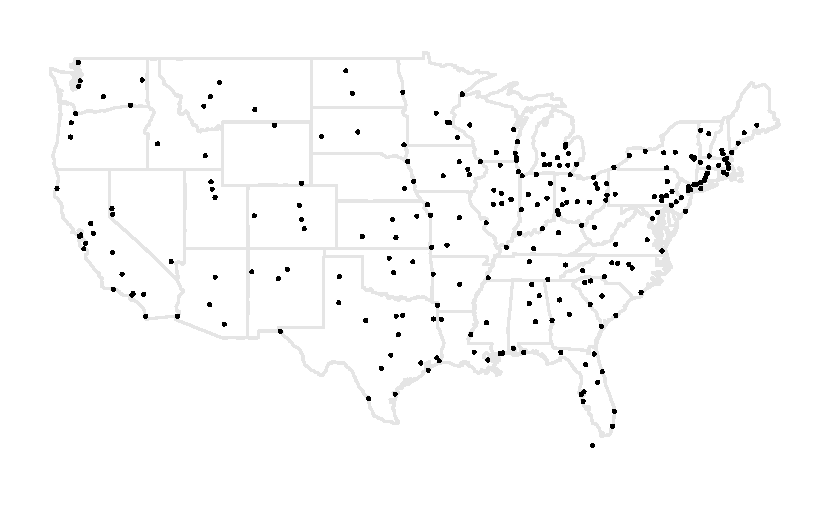
\includegraphics[keepaspectratio]{teodt-pq_files/figure-pdf/fig-map-1.pdf}}

}

\caption{\label{fig-map}257 American cites; our task is to find the
shortest path that goes through all of them.}

\end{figure}%

The task is to find the shortest path through those 257
cities.\footnote{The 257 cities are the cities in the lower 48 states
  from the 312 cities in North America that John Burkardt
  (\citeproc{ref-Burkhart2011}{2011}) mapped in his dataset USCA312.}

All nine of the decision theories I mentioned, and as far as I know
every competitor to them in the philosophical literature, say the thing
to do here is to draw whichever of the 256! possible paths is shortest.
That is not particularly helpful advice. Unless you know a lot about
problems like this, you can't draw the shortest path through the map.
And least, you can't draw it as such. You can't draw it in the way that
you can't enter the correct code on a locked phone
(\citeproc{ref-MandelkernEtAl2017}{Mandelkern, Schultheis, and Boylan
2017}).

One of the striking things about this puzzle is that it turns out there
are some helpful things that can be said. One helpful bit of advice to
someone trying to solve a problem like this is to use a Farthest
Insertion Algorithm.\footnote{To implement both this algorithm and the
  optimisation I'll mention below, I've used the TSP package by Michael
  Hashler and Kurt Hornik (\citeproc{ref-HashlerHornik2007}{2007}). The
  description of the two steps owes a lot to their summaries in the
  package documentation.} Insertion algorithms say to start with a
random city, then add cities to the path one at a time, at each time
finding the point to insert the city into the existing path that adds
the least distance. The Farthest Insertion Algorithm says that the city
added at each stage is the one farthest from the existing path.
Insertion algorithms in general produce pretty good paths in a very
short amount of time - at least on normal computers. And the Farthest
Insertion Algorithm is, most of the time, the best Insertion Algorithm
to use. Figure~\ref{fig-farthest} shows the result of one output of this
algorithm.\footnote{The algorithm is silent on which city you start
  with, and usually chooses this randomly.}

\begin{figure}

\centering{

\pandocbounded{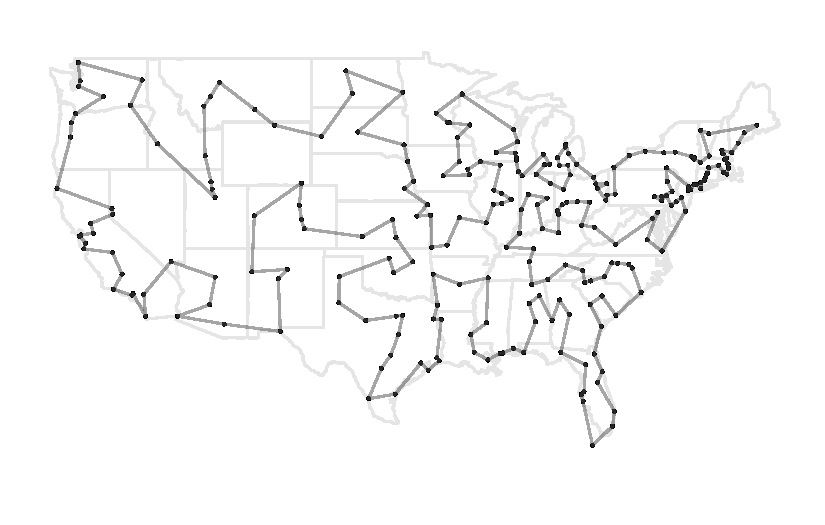
\includegraphics[keepaspectratio]{teodt-pq_files/figure-pdf/fig-farthest-1.pdf}}

}

\caption{\label{fig-farthest}An output of the Farthest Insertion
Algorithm, with a length of 21075 miles.}

\end{figure}%

The path in Figure~\ref{fig-farthest} is not bad, but with only a bit of
extra computational work, one can do better. A fairly simple
optimisation algorithm takes a map as input, and then deletes pairs of
edges at a time, and finds the shortest path of all possible paths with
all but those two edges. The process continues until no improvements can
be made by deleting two edges at a time, at which point you've found a
somewhat resilient local minimum. Figure~\ref{fig-two-opt} is the output
from applying this strategy to the path in Figure~\ref{fig-farthest}.

\begin{figure}

\centering{

\pandocbounded{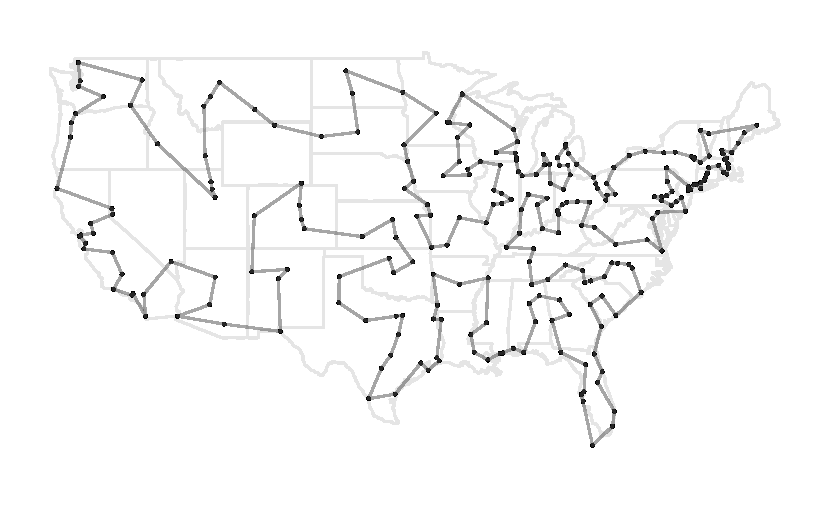
\includegraphics[keepaspectratio]{teodt-pq_files/figure-pdf/fig-two-opt-1.pdf}}

}

\caption{\label{fig-two-opt}The output of an optimisation process, which
reduced the path length to 20891 miles.}

\end{figure}%

This optimisation tends to produce paths that look a lot like the
original, but are somewhat shorter. For most practical purposes, the
best advice you could give someone faced with a problem like this is to
use a Farthest Insertion Algorithm, then optimise it in this way. Or, if
they have a bit more time, they could do this a dozen or so times, and
see if different starting cities led to slightly shorter paths.

While this is good advice, and indeed it's what most people should do,
it's not typically what is optimal to do. For that reason, it's not what
our nine decision theories would say to do. If one had unlimited and
free computing power available, hacks like these would be pointless. One
would simply look at all the possible paths, and see which was shortest.
I do not have free, unlimited computing power, so I didn't do this.
Using some black box algorithms I did not particularly understand, I was
able to find a shorter path, however. It took some time, both of mine
and my computer's, and for most purposes it would not have been worth
the hassle of finding it. Still, just to show it exists, I've plotted it
as Figure~\ref{fig-best}.

\begin{figure}

\centering{

\pandocbounded{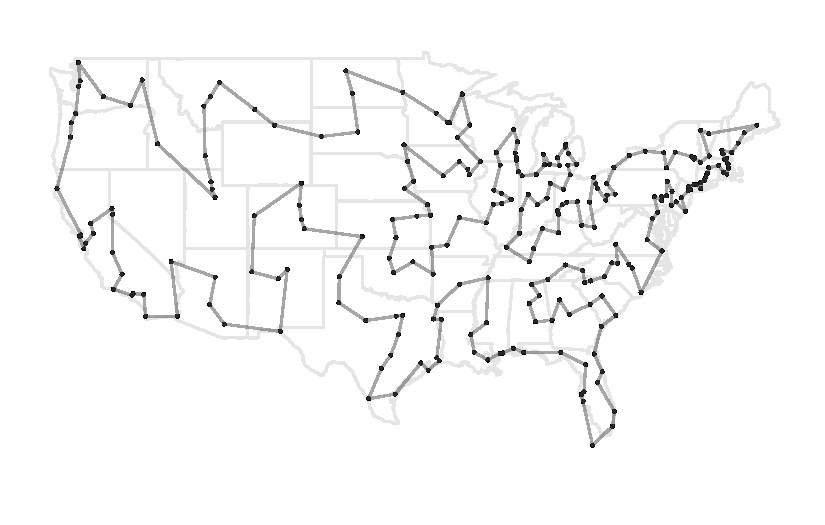
\includegraphics[keepaspectratio]{teodt-pq_files/figure-pdf/fig-best-1.pdf}}

}

\caption{\label{fig-best}The shortest path I could find, with a distance
of 20301 miles.}

\end{figure}%

I'm not sure if Figure~\ref{fig-best} is as short as possible, but I
couldn't find a shorter one. Still, for many purposes it wouldn't have
been worth the trouble it took to find this map.

\subsection{The Two Cases}\label{the-two-cases}

Table~\ref{tbl-examples} summarises the examples from the last two
sections.

\begin{longtable}[]{@{}lcc@{}}
\caption{How three approaches to decision theory handle the two
cases}\label{tbl-examples}\tabularnewline
\toprule\noalign{}
& Betting & Salesman \\
\midrule\noalign{}
\endfirsthead
\toprule\noalign{}
& Betting & Salesman \\
\midrule\noalign{}
\endhead
\bottomrule\noalign{}
\endlastfoot
Best outcome & Bet on winner & Shortest path \\
Decision theory & Pass & Shortest path \\
Best advice & Pass & Learn algorithms \\
\end{longtable}

The first row says which action would produce the best outcome in the
two cases. The third row says what advice one ought give someone who had
to choose in the two cases. And the middle row says what all the
decision theories say about the two cases. Notably, it agrees with
neither the first nor third row. Decision theory is neither in the
business of saying what will produce the best result, nor with giving
the most useful advice. So what is it doing?

\section{Decision Theory as
Idealisation}\label{decision-theory-as-idealisation}

Imagine a version of Chooser with, as Rousseau might have put it, their
knowledge as it is, and their computational powers as they might be.
That is, a version of Chooser who has unlimited, and free, computational
powers, but no more knowledge of the world than the actually have - save
what they learn by performing deductions from their existing knowledge.

Decision theories describe what that version of Chooser would do in the
problem that Chooser is facing. In the betting case, adding unlimited
computing power doesn't tell you who is going to win the game. So that
version of Chooser will still avoid betting. But in the Salesman case,
adding unlimited computing power is enough to solve the problem. They
don't even have to use any fancy techniques. To find the shortest path,
all it takes is finding the length of each path, and sorting the
results. The first requires nothing more that addition; at least if, as
was the case here, we provided the computer with the distances between
any pairs of cities as input. The second just requires being able to do
a bubble sort, which is technically extremely simple. To be sure, doing
all these additions, then doing a bubble sort on the results, will take
longer than most human lives on the kinds of computers most people have
available to them. But a version of Chooser with unlimited, free,
computational power will do these computations no problem at all.

If we say that Chooser should maximise expected utility, and we expect
them to compute that, then we're asking Chooser to perform a task that
is one step harder than calculating the shortest path in a Salesman
problem. To calculate an expected utility, for each option one looks up
a probability and a utility for each state\footnote{Exactly which
  probability it is, or indeed whether it even strictly is a
  probability, varies by which theory one chooses. But the basic idea
  that Chooser multiples something probability like by a utility is
  common across theories}, multiplies the two together, then adds the
results to get a value for the option. One repeats that for each state,
and finds an extreme value. Calculating the shortest path is exactly the
same, except one only has to look up one number (a distance) rather than
two (a probability and a utility), and there is no multiplication.
Solving for the shortest path is strictly easier than finding the
maximum expected utility. And yet finding the shortest path is
practically impossible.

This is one reason I focussed on Salesman problems rather than other
mathematical claims that Chooser is, in the standard models, assumed to
know. I didn't ask Chooser to bet on the Twin Primes conjecture. It's
possible one could come up with a model where finding the maximum
expected utility is typically possible but resolving the Twin Primes
conjecture is not; it's really hard to see how an agent who could always
calculate expected utilities couldn't solve a Salesman problem.

There are two other things that are distinctively interesting about this
problem which I'll simply note here, and defer longer discussion of them
to another day. First, it is possible to give practical useful advice
about how to solve Salesman problems. I've repeated some of the better
advice I've heard in the previous section. Second, when someone follows
this advice and does badly, as can happen with carefully designed maps,
it seems they are unlucky in just the same way that someone who
maximises expected utility but gets a low amount of actual utility is
unlucky. This raises some interesting questions about the normative
significance of expected utility maximisation that will be in the
background of the rest of the discussion here; hopefully I'll return to
them in later work.

At this point you might complain that I've talked about decision
theories asking Chooser to \emph{calculate} expected utilities. They do
no such thing. This is a point that Frank Knight made a century ago.

\begin{quote}
Let us take Marshall's example of a boy gathering and eating berries
\ldots{} We can hardly suppose that the boy goes through such mental
operations as drawing curves or making estimates of utility and
disutility scales. (\citeproc{ref-Knight1921}{Knight 1921, 66--67})
\end{quote}

And Knight does not say this is irrational. As long as the boy gets
enough berries, he's doing fine. In other terminology, we might say that
decision theory provides a criteria of rightness, not a deliberation
procedure.\footnote{I'm taking this distinction from Peter Railton
  (\citeproc{ref-Railton1984}{1984}), though his isn't the earliest use
  of the distinction. Alastair Norcross
  (\citeproc{ref-Norcross1997}{1997}) notes that the phrase ``criterion
  of rightness'' is used in the context of drawing this distinction by
  Sidgwick (\citeproc{ref-Sidgwick1907}{1907, bk. 4}, Chapter 1, §1).}
As long as one follows the rules of decision theory, even if one follows
them largely instinctually like Marshall's boy, one is rational.

This move just brings us back to the original problem. It's easy to
understand the distinction in Sidgwick. The criterion of rightness is
that one actually produces the best outcome. Which decision procedure
actually produces that outcome is hard to determine in advance, though
there are good reasons for suspecting that aiming for the best outcome
as such is not the optimal procedure. Why, however, should we think that
maximising \emph{expected} utility is a criteria of rightness? What
benefits does it have, over the standard of maximising actual utility,
as such a criteria? It is a somewhat easier rule to use, which makes it
a better deliberation procedure. Unfortunately, as the Salesman cases
show, there are other procedures that are better again qua deliberation
procedures too. So what benefit does it have?

One possible answer to this challenge is that expected utility
maximisation, or whatever one's favourite decision theory endorses, is a
goal; it is something we should try to achieve. On this picture,
decision theory is relevant because it tells us what idealised people
are like, and it recommends we try to be like them. In practice we can't
always be like them, as in the Salesman problem, but we should try.

The problem with this answer is that it is not, in general, good to try
to be like the ideal. The key point goes back to Lipsey and Lancaster's
\emph{General Theory of the Second Best}
(\citeproc{ref-LipseyLancaster}{Lipsey and Lancaster 1956}). Often
times, the right thing to do is something whose value consists in
mitigating the costs of our other flaws. It's not true in general,
indeed it's rather rare that it's true in practice, that approaches
which differ from the ideal in one respect are better than all
approaches which differ from the ideal in two respects. For example, us
non-ideal agents should, especially in high stakes settings, stop and
have a little think before acting. The ideal agent of decision theory
never stops to have a think. After all, stopping is costly, and the
ideal agent gets no gain from incurring that cost.

In general, we differ from the ideal agent in any number of ways. Some
of these are respects in which we'd be better off being more like them.
For example, they correctly hedge against costly but realistic risks.
But some of these are respects in which we'd be worse off being more
like them. For instance, they never stop to have a think, or put in
effort to get better at calculations. Knowing that the ideal agent is
\emph{F} doesn't tell us whether we should try to be \emph{F} unless we
also know that \emph{F} is more like hedging rather than more like never
trying to get better at calculating. That, unfortunately, is not
something which we can really figure out from within the idealised
approach to decision theory that is standard these days.

\section{Idealisations as Models}\label{idealisations-as-models}

At the start I said that the word `idealised' gets used differently in
ethics and in philosophy of science. The main claim I want to make in
this section is that we should understand the idealisations in decision
theory in the latter sense. In particular, we should understand them as
simplifications. Michael Weisberg (\citeproc{ref-Weisberg2007}{2007})
identifies three kinds of idealisations in science: Galilean, which
distort the situation to make computation easier; minimalist, which only
include the factors one takes to be causally significant to a situation;
and multiple models, where one tries to understand a situation by
considering different minimal idealisations with different strengths and
weaknesses. The idealisations in decision theory are the second kind.
They aren't particularly computationally tractable, unlike the Galilean
idealisations, and there is typically just the one of them.

Another way to put this is that the idealisations in, say, ideal gas
theory are \emph{simplifications} rather than \emph{perfections}. We do
not think that having volume is an imperfection. Maybe some religious
traditions think this, but it isn't baked into introductory chemistry.
Nor do we think that they are things we should aim for. Introductory
chemistry does not imply a \emph{Smaller the better!} rule for
molecules. Rather, it says that volumeless molecules with perfectly
elastic collisions are simpler to work with, and that some of the
phenomena of real gases can be explained by looking at this simpler
model.

Decision theory is engaged in the same kind of project. Just like the
point masses we use in the ideal gas law, they say not what should
happen, but what would happen in the absence of certain complications.
The idealisation here is not a perfection, for two reasons. First,
allocating zero seconds to hard but important math problems is not a
perfection, it's a practical vice. Yet it's what the ideal agent does.
Second, the idealised self is not in fact absolutely perfect. They have
similar informational limitations to what we do.

This is the point of the basketball example. The idealised self that
gets used in decision theory is god-like god-like in one respect -
computational ability - but human-like in another - informational
awareness. That's a common feature of idealised models; one doesn't
idealised away from absolutely everything.

Why do we use these models? Part of the answer here comes back to the
much discussed question of why we use models at all. I'm going to assume
that part of the answer is that minimal models are explanatorily
powerful when the difference between the minimal model and reality is
not relevant to predicting, explaining, or understanding what happens in
the real world. So my hypothesis is that the idealised models of
decision theory are, at least sometimes, relevant to predicting,
explaining, or understanding what happens in the real world.

It's tempting to identify the situations where decision theory is
relevant with high stakes situations. After all, in high-stakes
situations deciders are disposed to throw enough computational resources
at the problem that the differences between ordinary people and ideal
agents shrinks. But that is isn't quite right. After all, in many high
stakes cases, the decider also throws enough investigative resources at
the problem that holding actual knowledge fixed is a bad modelling
assumption.

To find a case where decision theory is relevant, we need are cases
where there are principled limitations to the decider's informational
capacities. There are two kinds of cases that are relevant here. One is
where the information concerns the future, and the decision must be made
now. And the other is where the information that someone else has (or at
least may have) just as much incentive to suppress the information as
the decider has to find it. Most textbook examples of the usefulness of
decision theory concern the first kind, though they don't always make
explicit why it matters that the case is future directed. I'm going to
work through a case of the second kind that I think is enlightening
about the way decision theory is valuable.

Until very recently, used cars sold at a huge discount to new cars, even
when the cars were just a few months old with almost no usage. For a
long time there was no agreed upon explanation for this phenomena. The
most common theory was that it reflected a preference, or perhaps a
prejudice, on the part of buyers. George Akerlof
(\citeproc{ref-Akerlof1970}{1970}) showed how this discount could be
explained in a model of perfectly rational agents. His model makes the
following assumptions.

\begin{enumerate}
\def\labelenumi{\arabic{enumi}.}
\tightlist
\item
  Cars vary a lot in quality, even cars that come from the same
  production line.
\item
  Sellers of used cars know how good the particular car they are selling
  is.
\item
  Buyers of used cars do not know how good the car is; they only know
  how good that model of cars generally is.
\item
  People rarely sell cars they just bought.
\item
  Everyone involved is an expected utility maximiser.
\end{enumerate}

Based on these five assumptions, Akerlof built a formal model of the
market for recently used cars. In the model, the most common reason to
sell a car one just bought is the discovery that it was a bad instance
of that kind of car. Knowing this, buyers of used cars demanded a big
discount in exchange for the possibility they were buying a dud. But as
long as there are enough forced sellers of good recently purchased cars,
who prefer whatever money they can get for their car to keeping the car,
there can be an equilibrium where lightly used cars sell at a heavy
discount to new cars, and it is rational for (some) owners to sell into
this market, and for (some) buyers to buy in this market.

If Akerlof was right, and I think he was largely correct, you'd expect
the used car discount to fall if either of the following things
happened. First, it would fall if production lines got more reliable,
and cars off the same line were more similar to one another. And second,
it would fall if buyers had access to better tools\footnote{Better that
  is than a drive around the block test drive.} to judge the quality of
used cars. By 2020 both of those things had happened, and the used car
discount was almost zero.\footnote{Then during the pandemic very strange
  things happened in the used car market and the `discount' arguably
  went negative. Whatever was happening there was not explained by the
  Akerlof model.}

The philosophical significance of this is that one can't build models
like Akerlof's without a theory of rational action under uncertainty.
The big payoff of philosophical decision theory is that it's an
essential input to useful models, like the Akerlof model. Since those
models are useful, getting the inputs to them right is useful.

\section{Conclusions}\label{conclusions}

This has largely been a work of meta-philosophy. I've argued that
decision theorists are building idealisations in the sense of simple
models. And I've argued that this is a good project not because it
issues in advice, or evaluation, but because it provides inputs to
explanations. In particular, decision theoretic explanations are often
accurate when people can behave somewhat like computationally ideal
agents, but must still behave like informationally limited agents.

If I'm right, there are several consequences for first-order decision
theory. I'll end the paper going over four of them.

\subsection{The Value of Limited
Theories}\label{the-value-of-limited-theories}

We use different styles of explanations for different phenomena. If a
product routinely sells for \$7.99, we might use a rational choice
explanation for why the price is roughly \$8 rather than roughly \$10,
and then a very different kind of explanation for why it is \$7.99
rather than \$8.01. It isn't always a weakness of an explanation that it
does not generalise to as many cases as one might have hoped.

This matters for decision theory. If a decision theory goes silent on a
certain kind of case, that isn't necessarily a bad thing. One sometimes
hears theorists talk as if the fact that a theory doesn't say what to do
in a particular situation is very bad, because the point of decision
theory is to provide advice. But if decision theory goes silent on cases
where we don't think decision theoretic explanations are likely to be
good, that's not necessarily a bad thing.

\subsection{The Ideal Agent}\label{the-ideal-agent}

I've left off a lot of details about exactly what the ideal agent is
like. I said they are computationally good, but informationally limited.
This leaves open a lot of questions. Do they have perfect information
about their own beliefs and desires, or about their own plans? Are they
able to stick to a plan, and if so, which kinds of plans can they stick
to?

One way to try answering these questions is by asking whether the
inability to know one of these things, or do one of these things, is a
kind of imperfection. If it is, we've discovered a new feature of the
ideal, perfect agent.

If I'm right, that's the wrong way to go about answering the question.
We should ask instead if assuming that the ideal decider has these
features makes them too dissimilar to real people for explanatory
purposes. For instance, I think we should allow that ideal deciders can
play mixed strategies, because being able to play mixed strategies does
not make the ideal decider that different to real people. In
circumstances where real deciders have sufficient computational
resources that ideal deciders are good models for them, real deciders
also have sufficient resources to play mixed strategies.

Whether I'm right or wrong about mixed strategies, the point I want to
really stress is the approach to answering these questions about
idealisations. The right idealisation does not describe what we should
be like, but rather what it is helpful to model us as being like.

\subsection{Non-Ideal Theory}\label{non-ideal-theory}

If actual decision theory is a kind of ideal theory, that means there is
a space for a non-ideal theory. And there are a bunch of interesting
philosophical questions about it. I think the right non-ideal theory
will be some kind of reliabilism. Even if that's right, it hardly
settles matters. There are, after all, many different kinds of
reliabilism, and we'd need to have answers to the decision theoretic
equivalents of the generality problem, and the new evil demon problem.
Still, these feel like answerable questions, and there are interesting
projects to work on here.

\subsection{Reconciliation}\label{reconciliation}

If two types of theory exist, both ideal and non-ideal, some
reconciliation possibilities open up. Perhaps the right thing to say
about Newcomb's Problem is that there is a sense in which one should
take one box, and there is a sense in which one should take two boxes.
One way to get this result would be to endorse the following three
claims.

\begin{enumerate}
\def\labelenumi{\arabic{enumi}.}
\tightlist
\item
  The right ideal decision theory is some broadly causal decision
  theory.
\item
  The right non-ideal decision theory is some kind of reliabilism.
\item
  In Newcomb's Problem, one boxers and two boxers are in the same
  reference class, so the right thing to do is the thing that, on
  average, produces the best results in that large class.
\end{enumerate}

I don't want to endorse all these; I'm particularly sceptical of 3. The
point is just that when we distinguish ideal from non-ideal theories we
open up some new options in what might seem like stale debates.

\subsection{Other Idealisations}\label{other-idealisations}

The most interesting question that opens up from this way of thinking
about decision theory is whether we could develop any other
idealisations that are explanatorily powerful. As Weisberg notes, an
important kind of idealisation involves developing many models that help
explain different phenomena. Here that might involve changing what
information the ideal agent has, or what computational powers they have.

In economics there has been some interesting projects along these lines.
One that's particularly relevant here is the development of cursed
equilibrium models (Eyster and Rabin
(\citeproc{ref-EysterRabin2005}{2005})). In cursed equilibrium models,
agents maximise expected utility with respect to some information, but
not the information they actually have. In particular, they don't always
take fully into account what they can figure out about other people's
information from observing the acts other people perform. It's a bit
more complicated than this in practice, but roughly it's as if people
ignore what other people are doing.

These models are relevant here for two reasons. One is that the main
example I used of decision theory working, Akerlof's model for used
cars, involved people making just the kind of inference that they do not
make in cursed equilibrium models. The reason the used car market
settles at such a discount, in an Akerlof model, is that buyers reason
from the fact that sellers are choosing to sell that sellers have
private information. That inference, from observed behaviour to
conclusions about the private information the other person has, is
exactly what agents do not make in cursed equilibrium models. This
matters because in a bunch of experimental settings, cursed equilibrium
models make more accurate predictions than rational choice models.

This doesn't on its own show the Akerlof explanation is wrong. It might
just show that explanation was incomplete. To complete the explanation
we could simply add the premises that cars are expensive, and that
people act more carefully when making expensive purchases. The first
premise is clearly true, cars are indeed expensive, and there is some
evidence for the second. Still, thinking about cursed equilibrium
models, which are still incredibly idealised, helps both explain new
phenomena, and appreciate more fully the explanations that rational
choice models make.

Cursed equilibrium models have not been developed nearly as fully as
rational choice models; it's only very recently that fully dynamic
versions of them have been put forward (\citeproc{ref-CohenLi2023}{Cohen
and Li 2023}; \citeproc{ref-Fong2023}{Fong, Lin, and Palfrey
forthcoming}). I certainly don't want to say this is the only way to
modify the idealisations in standard decision theory, or even the best
such way. What I do want to say is that thinking about decision theory
as the project of building good simplified models suggests that the
project of building multiple models of decision could have some value.

\subsection*{References}\label{references}
\addcontentsline{toc}{subsection}{References}

\phantomsection\label{refs}
\begin{CSLReferences}{1}{0}
\bibitem[\citeproctext]{ref-Ahmed2014}
Ahmed, Arif. 2014. \emph{Evidence, Decision and Causality}. Cambridge:
{C}ambridge {U}niversity {P}ress.

\bibitem[\citeproctext]{ref-Akerlof1970}
Akerlof, George. 1970. {``The Market for "Lemons": Quality Uncertainty
and the Market Mechanism.''} \emph{Quarterly Journal of Economics} 84
(3): 488--500. \url{https://doi.org/10.2307/1879431}.

\bibitem[\citeproctext]{ref-BuchakRisk}
Buchak, Lara. 2013. \emph{Risk and Rationality}. Oxford: Oxford
University Press.

\bibitem[\citeproctext]{ref-Burkhart2011}
Burkardt, John. 2011. {``Cities.''}
\url{https://people.sc.fsu.edu/~jburkardt/datasets/cities/cities.html}.

\bibitem[\citeproctext]{ref-CohenLi2023}
Cohen, Shani, and Shengwu Li. 2023. {``Sequential Cursed Equilibrium.''}
2023. \url{https://arxiv.org/abs/2212.06025}.

\bibitem[\citeproctext]{ref-EysterRabin2005}
Eyster, Erik, and Matthew Rabin. 2005. {``Cursed Equilibrium.''}
\emph{Econometrica} 73 (5): 1623--72.
\href{https://10.1111/j.1468-0262.2005.00631.x}{10.1111/j.1468-0262.2005.00631.x}.

\bibitem[\citeproctext]{ref-Fong2023}
Fong, Meng-Jhang, Po-Hsuan Lin, and Thomas R. Palfrey. forthcoming.
{``Cursed Sequential Equilibrium.''} \emph{American Economic Review},
forthcoming.

\bibitem[\citeproctext]{ref-Fusco2024}
Fusco, Melissa. 2024. {``Absolution of a Causal Decision Theorist.''}
\emph{No{û}s} 58 (3): 616--43. \url{https://doi.org/10.1111/nous.12459}.

\bibitem[\citeproctext]{ref-Gallow2020}
Gallow, J. Dmitri. 2020. {``The Causal Decision Theorist's Guide to
Managing the News.''} \emph{The Journal of Philosophy} 117 (3): 117--49.
\url{https://doi.org/10.5840/jphil202011739}.

\bibitem[\citeproctext]{ref-GibbardHarper1978}
Gibbard, Allan, and William Harper. 1978. {``Counterfactuals and Two
Kinds of Expected Utility.''} In \emph{Foundations and Applications of
Decision Theory}, edited by C. A. Hooker, J. J. Leach, and E. F.
McClennen, 125--62. Dordrecht: Reidel.

\bibitem[\citeproctext]{ref-HashlerHornik2007}
Hahsler, Michael, and Kurt Hornik. 2007. {``TSP---Infrastructure for the
Traveling Salesperson Problem.''} \emph{Journal of Statistical Software}
23 (2): 1--21. \url{https://doi.org/10.18637/jss.v023.i02}.

\bibitem[\citeproctext]{ref-Joyce1999}
Joyce, James M. 1999. \emph{The Foundations of Causal Decision Theory}.
Cambridge: Cambridge University Press.

\bibitem[\citeproctext]{ref-Knight1921}
Knight, Frank. 1921. \emph{Risk, Uncertainty and Profit}. Chicago:
University of Chicago Press.

\bibitem[\citeproctext]{ref-LevinsteinSoares2020}
Levinstein, Benjamin Anders, and Nate Soares. 2020. {``Cheating Death in
Damascus.''} \emph{Journal of Philosophy} 117 (5): 237--66.
\url{https://doi.org/10.5840/jphil2020117516}.

\bibitem[\citeproctext]{ref-Lewis1981b}
Lewis, David. 1981. {``Causal Decision Theory.''} \emph{Australasian
Journal of Philosophy} 59 (1): 5--30.
\url{https://doi.org/10.1080/00048408112340011}.

\bibitem[\citeproctext]{ref-Lewis1994b}
---------. 1994. {``Reduction of Mind.''} In \emph{A Companion to the
Philosophy of Mind}, edited by Samuel Guttenplan, 412--31. Oxford:
Blackwell. \url{https://doi.org/10.1017/CBO9780511625343.019}.

\bibitem[\citeproctext]{ref-Lewis-Gorman-19041989}
---------. (1989) 2020. {``Letter to Jonathan Gorman, 19 April 1989.''}
In \emph{Philosophical Letters of David {K}. Lewis}, edited by Helen
Beebee and A. R. J. Fisher, 2:472--73. Oxford: Oxford University Press.

\bibitem[\citeproctext]{ref-LipseyLancaster}
Lipsey, R. G., and Kelvin Lancaster. 1956. {``The General Theory of
Second Best.''} \emph{Review of Economic Studies} 24 (1): 11--32.
\url{https://doi.org/10.2307/2296233}.

\bibitem[\citeproctext]{ref-MandelkernEtAl2017}
Mandelkern, Matthew, Ginger Schultheis, and David Boylan. 2017.
{``Agentive Modals.''} \emph{Philosophical Review} 126 (3): 301--43.
\url{https://doi.org/10.1215/00318108-3878483}.

\bibitem[\citeproctext]{ref-Norcross1997}
Norcross, Alastair. 1997. {``Consequentialism and Commitment.''}
\emph{Pacific Philosophical Quarterly} 78 (4): 380--403.
\url{https://doi.org/10.1111/1468-0114.00045}.

\bibitem[\citeproctext]{ref-Podgorski2022}
Podgorski, Aberlard. 2022. {``Tournament Decision Theory.''}
\emph{No{û}s} 56 (1): 176--203.
\url{https://doi.org/10.1111/nous.12353}.

\bibitem[\citeproctext]{ref-Railton1984}
Railton, Peter. 1984. {``Alienation, Consequentialism, and the Demands
of Morality.''} \emph{Philosophy and Public Affairs} 13 (2): 134--71.

\bibitem[\citeproctext]{ref-Robinson1949}
Robinson, Julia. 1949. {``On the Hamiltonian Game (a Traveling Salesman
Problem).''} Santa Monica, CA: The RAND Corporation.

\bibitem[\citeproctext]{ref-Roussos2022}
Roussos, Joe. 2022. {``Modelling in Normative Ethics.''} \emph{Ethical
Theory and Moral Practice} 25: 865--89.
\url{https://doi.org/10.1007/s10677-022-10326-4}.

\bibitem[\citeproctext]{ref-Roussos2025}
---------. 2025. {``Normative Formal Epistemology as Modelling.''}
\emph{British Journal for the Philosophy of Science} 76 (2): 421--48.
\href{https://doi.org/10.1086/718493\%20}{https://doi.org/10.1086/718493
}.

\bibitem[\citeproctext]{ref-Schrijver2005}
Schrijver, Alexander. 2005. {``On the History of Combinatorial
Optimization (till 1960).''} \emph{Handbooks in Operations Research and
Management Science} 12: 1--68.
\url{https://doi.org/10.1016/S0927-0507(05)12001-5}.

\bibitem[\citeproctext]{ref-Sidgwick1907}
Sidgwick, Henry. 1907. \emph{The Methods of Ethics}. Seventh. London:
Macmillan.

\bibitem[\citeproctext]{ref-Skyrms1990}
Skyrms, Brian. 1990. \emph{The Dynamics of Rational Deliberation}.
Cambridge, MA: Harvard University Press.

\bibitem[\citeproctext]{ref-Spencer2021}
Spencer, Jack. 2021. {``An Argument Against Causal Decision Theory.''}
\emph{Analysis} 81 (1): 52--61.
\url{https://doi.org/10.1093/analys/anaa037}.

\bibitem[\citeproctext]{ref-wiki-salesman}
Travelling salesman problem. 2024. {``Travelling Salesman Problem---
{W}ikipedia{,} the Free Encyclopedia.''}
\url{https://en.wikipedia.org/w/index.php?title=Travelling_salesman_problem&oldid=1209291065}.

\bibitem[\citeproctext]{ref-Wedgwood2013a}
Wedgwood, Ralph. 2013. {``Gandalf's Solution to the Newcomb Problem.''}
\emph{Synthese} 190 (14): 2643--75.
\url{https://doi.org/10.1007/s11229-011-9900-1}.

\bibitem[\citeproctext]{ref-Weisberg2007}
Weisberg, Michael. 2007. {``Three Kinds of Idealization.''} \emph{The
Journal of Philosophy} 104 (12): 639--59.
\url{https://doi.org/10.5840/jphil20071041240}.

\end{CSLReferences}




\end{document}
